%%%%%%%%%%%%%%%%%%%%%%%%%%%%%%%%%%%%%%%%%%%%%%%%%%%%%%%%%%%%%%%%%
%2345678901234567890123456789012345678901234567890123456789012345
%        1         2         3         4         5         6     
\chapter{Mobile robot control framework}
\label{cha:framework}
A mobile robot is a complex system with several functional block. From control perspect of view, the system can be roughly divided into 2 parts, global planner and local planner.
The global planner, which is responsible to sense the environment and make decision to plan the trajectory is out of scope of this paper, we just simplify it as a node which  output task space command at 20Hz.
Our focus in this study is on the other part, local planner, which takes the task space velocity and acceleration command $\dot{\xi},\ddot{\xi}$ as input and calculate the corresponding optimal joint response, 
coordinate the steering and driving of four wheels, Which include 4 steering motors and 4 driving motors. 
The local planner communicate with these motors with CAN bus at 1 KHz, and take the task space command from global planner with ROS network at the same time.
Inside the local planner, we deployed 2 sets of control logic, ICR optimization control\cref{cha:ICR} and approximation based inverse kinematic control\cref{cha:inverseKinematics}. A Switching mechanism is used to decide
which method is to be used given the status the platform is in.



%%%%%%%%%%%%%%%%%%%%%%%%%%%%%%%%%%%%%%%%%%%%%%%%%%%%%%%%%%%%%%%%%%%%%%%%%%%%%%%%%%%%%%%%%%%%%%%%%%%%%%%%%%%%%%%%%%%%%%%%%%%%%%%%%%%%%%%%%%%%%%%%%%%%%%%%%%%%%%%%%%%%%%%%%%%%%%%%%%%%%%%%%%%%%%%%

\tikzstyle{myarrow}=[->, thick]
\tikzstyle{line}=[-, thick]
\begin{figure}[t]\label{fig:hardwareStructure}
	\begin{center}
		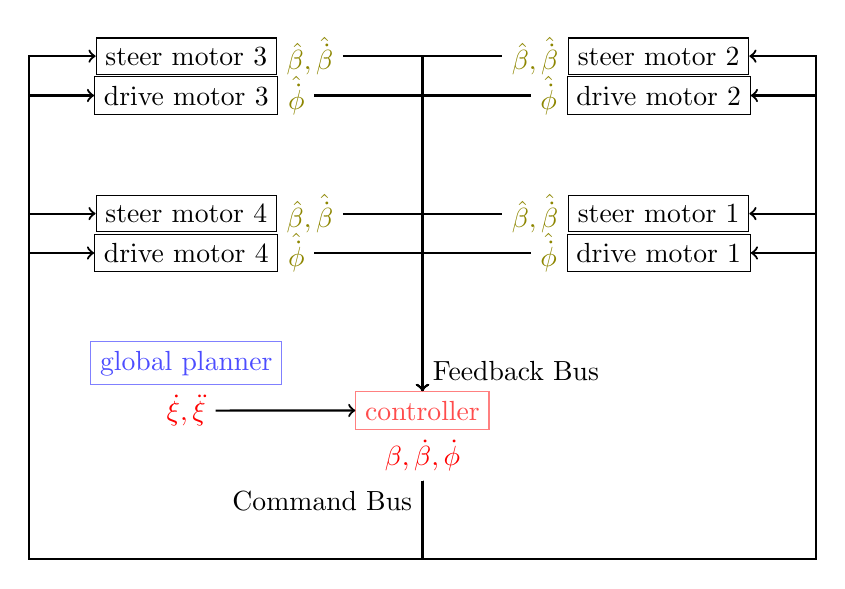
\begin{tikzpicture}
		    \node (global planner) at (-3, 0.6) [rectangle, draw=blue!50, text=blue!70, label={[name=task command, red]-90:$\dot{\xi},\ddot{\xi}$}] {global planner};
		    \node (controller) at (0, 0) [rectangle, draw=red!50, text=red!70, label={[name=command, red]-90:$\beta,\dot{\beta},\dot{\phi}$}] {controller};
		    
			\node (steer1) at (3, 2.5) [rectangle, draw=black, label={[name=steer1Feedback, olive]180:$\hat{\beta},\hat{\dot{\beta}}$}] {steer motor 1};
			\node (drive1) at (3, 2) [rectangle, draw=black, label={[name=drive1Feedback, olive]180:$\hat{\dot{\phi}}$}] {drive motor 1};
			\draw[myarrow] (steer1Feedback) -| (controller.north);
			\draw[line] (drive1Feedback) -| (controller.north);

            \node (steer2) at (3, 4.5) [rectangle, draw=black, label={[name=steer2Feedback, olive]180:$\hat{\beta},\hat{\dot{\beta}}$}] {steer motor 2};
			\node (drive2) at (3, 4) [rectangle, draw=black, label={[name=drive2Feedback, olive]180:$\hat{\dot{\phi}}$}] {drive motor 2};
			\draw[myarrow] (steer2Feedback) -| (controller.north);
			\draw[line] (drive2Feedback) -| (controller.north);
			
			\node (steer3) at (-3, 4.5) [rectangle, draw=black, label={[name=steer3Feedback, olive]0:$\hat{\beta},\hat{\dot{\beta}}$}] {steer motor 3};
			\node (drive3) at (-3, 4) [rectangle, draw=black, label={[name=drive3Feedback, olive]0:$\hat{\dot{\phi}}$}] {drive motor 3};
			\draw[myarrow] (steer3Feedback) -| (controller.north);
			\draw[line] (drive3Feedback) -| (controller.north);
			
			\node (steer4) at (-3, 2.5) [rectangle, draw=black, label={[name=steer4Feedback, olive]0:$\hat{\beta},\hat{\dot{\beta}}$}] {steer motor 4};
			\node (drive4) at (-3, 2) [rectangle, draw=black, label={[name=drive4Feedback, olive]0:$\hat{\dot{\phi}}$}] {drive motor 4};
			\draw[myarrow] (steer4Feedback) -| (controller.north);
			\draw[line] (drive4Feedback) -| (controller.north) node[anchor=south west] {Feedback Bus};
			
			\draw[myarrow] (command.south) -- ++ (0,-1) -- ++(5,0)-- ++(0, 2) |- (steer1.east);
			\draw[myarrow] (command.south) -- ++ (0,-1) -- ++(5,0)-- ++(0, 2) |- (drive1.east);
			\draw[myarrow] (command.south) -- ++ (0,-1) -- ++(5,0)-- ++(0, 2) |- (steer2.east);
			\draw[myarrow] (command.south) -- ++ (0,-1) -- ++(5,0)-- ++(0, 2) |- (drive2.east);
			\draw[myarrow] (command.south) -- ++ (0,-1) -- ++(-5,0)-- ++(0, 2) |- (steer3.west);
			\draw[myarrow] (command.south) -- ++ (0,-1) -- ++(-5,0)-- ++(0, 2) |- (drive3.west);
			\draw[myarrow] (command.south) -- ++ (0,-1) -- ++(-5,0)-- ++(0, 2) |- (steer4.west);
			\draw[myarrow] (command.south) node[anchor=north east] {Command Bus} -- ++ (0,-1) -- ++(-5,0)-- ++(0, 2) |- (drive4.west);
			\draw[myarrow] (task command)--(controller.west);
		\end{tikzpicture}
	\end{center}
	\caption{System inter-connection}
\end{figure}


%%%%%%%%%%%%%%%%%%%%%%%%%%%%%%%%%%%%%%%%%%%%%%%%%%%%%%%%%%%%%%%%%%%%%%%%%%%%%%%%%%%%%%%%%%%%%%%%%%%%%%%%%%%%%%%%%%%%%%%%%%%%%%%%%%%%%%%%%%%%%%%%%%%%%%%%%%%%%%%%%%%%%%%%%%%%%%%%%%%%%%%%%%%%%%%%

\section{Low-level controller structure}
\label{sec:structure}
\tikzstyle{myarrow}=[->, thick]
\tikzstyle{line}=[-, thick]
The low-level controller is consist of 4 major functional blocks. The 2 control logic blocks are the most essential blocks in this controller, they each are suitable for handling a certain scenario and thus only 
one of them would be enabled at each time instance. The enable signal is produced by the switching mechanism beased on the current status of the platform, which would be detailed explained in \cref{subsec:switching}.
The forward kinematic block takes the wheel sensor/encoder feedback and calculate the current platform task space speed $\hat{\dot{\xi}} $, which would be taken by 2 control logic blocks as input and also by 
switching block as platform current state. The control sequence flow is illustrated in figure \cref{fig:controller} .
\begin{figure}[t]\label{fig:controller}
	\begin{center}
		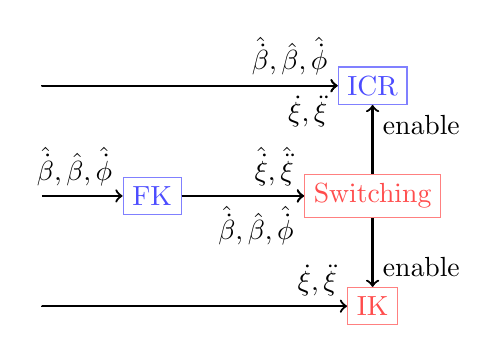
\begin{tikzpicture}[scale=0.7]

			
		    \node (FKAM) at (-2, 0) [rectangle, draw=blue!50, text=blue!70] {FK};
		    \node (switch) at (2, 0) [rectangle, draw=red!50, text=red!70] {Switching};
		    \node (ICR) at (2, 2) [rectangle, draw=blue!50, text=blue!70] {ICR };
		    \node (IKAM) at (2, -2) [rectangle, draw=red!50, text=red!70] {IK};
			
			\draw[myarrow] (-4, 2) |-(ICR.west) node [anchor=south east]{$\hat{\dot{\beta}},\hat{\beta},\hat{\dot{\phi}}$};
			\draw[myarrow] (-4, 0) --(FKAM.west) node [anchor=south east]{$\hat{\dot{\beta}},\hat{\beta},\hat{\dot{\phi}}$};
			\draw[myarrow] (-4, -2) |-(IKAM.west) node [anchor=south east]{$\dot{\xi},\ddot{\xi}$};
			\draw[myarrow] (-4, 2) |-(ICR.west) node [anchor=north east]{$\dot{\xi},\ddot{\xi}$};
			\draw[myarrow] (FKAM) --(switch.west) node [anchor=south east]{$\hat{\dot{\xi}},\hat{\ddot{\xi}}$};
            \draw[myarrow] (FKAM) --(switch.west) node [anchor=north east]{$\hat{\dot{\beta}},\hat{\beta},\hat{\dot{\phi}}$};
            \draw[myarrow] (switch.north) -- (ICR.south) node [anchor=north west]{enable};
            \draw[myarrow] (switch.south) --(IKAM.north) node [anchor=south west]{enable};
		\end{tikzpicture}
	\end{center}
	\caption{Low-level controller structure}
\end{figure}
%%%%%%%%%%%%%%%%%%%%%%%%%%%%%%%%%%%%%%%%%%%%%%%%%%%%%%%%%%%%%%%%%%%%%%%%%%%%%%%%%%%%%%%%%%%%%%%%%%%%%%%%%%%%%%%%%%%%%%%%%%%%%%%%%%%%%%%%%%%%%%%%%%%%%%%%%%%%%%%%%%%%%%%%%%%
\subsection{Switching mechanism}
\label{subsec:switching}
The two control logic each has advantages. 
The idea of approximation based inverse kinematic control is to linearize the complex and highly non-linear kinematic system at each control instance, so that we treat it as a linear system and thus capable to scaling down the task space command $\dot{\xi}, \ddot{\xi}$ whenever it occurs inconsistency. However, the accuracy of the approximation varies. It is very precise when the $ICR_{reference}$ is relative far away from the platform. The accuracy decrease when the  $ICR_{reference}$ gets closer. The approximation error goes to peak when the $ICR_{reference}$ is close to the four wheel axes and body frame origin, which is shown in \cref{fig:approximationError}. These five points are called singular points and are all within a small region centered at body frame origin. 
\begin{figure}[!ht]
    \centering
    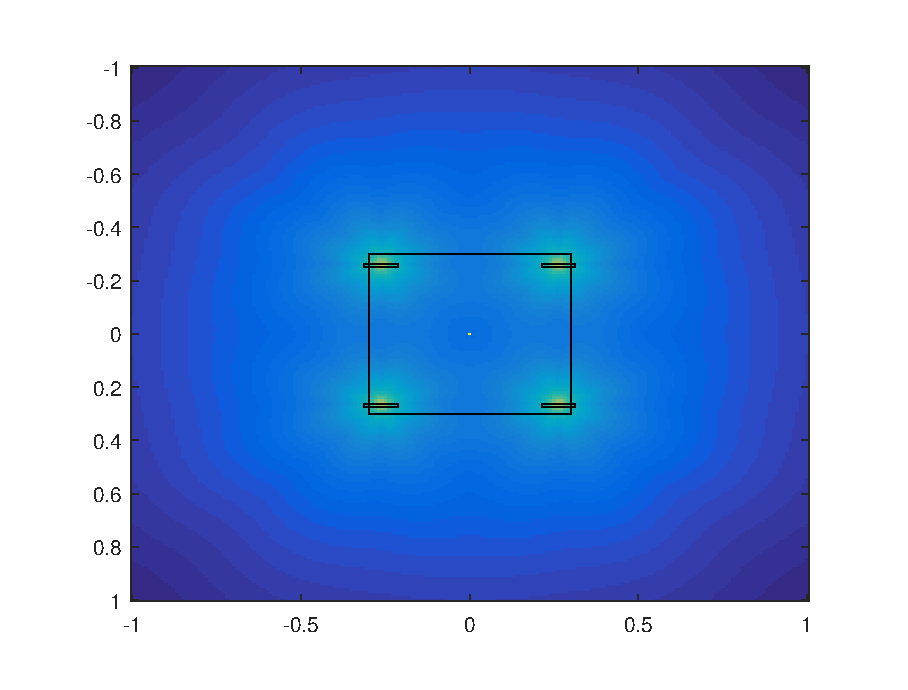
\includegraphics[width=0.75\textwidth]{Figures/approximationError.eps}
    \caption{Approximation error regarding ICR position}
    \label{fig:approximationError}
\end{figure}
However, the ICR optimization control strategy is much more better on handling the case when ICR is close to the platform, while the accuracy will decrease as ICR moves far away, especially when the platform is doing pure translation, which means ICR is infinit far away.

These 2 strategy are complementary to each other. So we set up a simply logic to switch between them, 
\begin{itemize}
    \item[1.] Firstly estimate the current ICR position based on the wheel steering feedback from sensors. this does not need to be very accurate, so we just take the pair of wheels which have the biggest steering angle difference and calculate the $ICR_{current}$ by the intersection of their zero motion line ($\overrightarrow{x^{wi}}$).
    \item[2.] If the $ICR_{current}$ is larger than a pre-set threshold, we choose to use the approxima-tion based inverse kinematic control. Otherwise the ICR optimization method would be chosen.
\end{itemize}